\documentclass[12pt,a4paper,utf8]{ctexart}
\usepackage{ctex,amsmath,amssymb,subfig,cite,graphicx,diagbox,fontspec,fancyhdr,geometry}
\usepackage[ntheorem]{empheq}
\usepackage{enumitem,fullpage,cleveref,cellspace,listings,color,framed}
\definecolor{gray}{rgb}{0.5,0.5,0.5}
\definecolor{dkgreen}{rgb}{.068,.578,.068}
\definecolor{dkpurple}{rgb}{.320,.064,.680}

%set Fortran styles
\lstset{
    frameround=tftf,
    language=Fortran,
    keywords={SELECT,PROGRAM,PRINT,STOP,END,WRITE,INTEGER,REAL,COMPLEX,CHARACTER,LOGICAL,READ,FORMAT,IMPLICIT,PARAMETER,DATA,EQUIVALENCE,TYPE,PAUSE,CONTINUE,CYCLE,EXIT,IF,SELECT,DO,ALLOCATE,DEALLOCATE,WHERE,FORALL,SUBROUTIHNE,CALL,RETURN,FUNCTION,COMMON,BLOCK DATA,SAVE,INTERFACE,CONTAIN,MODULE,USE,PUBLIC,PRIVATE,ENTRY,OPEN,INQUIRE,CLOSE,NAMELIST,POINTER,NULLFY,REWIND,BACKSPACE,ENDFILE
    },
    basicstyle=\small\ttfamily,
    numbers=left,
    numberstyle=\small,
    keywordstyle=\color{blue}\bfseries,
    commentstyle=\color{dkgreen},
    stringstyle=\color{dkpurple},
    backgroundcolor=\color{white},
    tabsize=2,
    showspaces=false,
    showstringspaces=false,
    breaklines=true,
    frame=trBL,
}
\CTEXsetup[format+={\raggedright}]{section}
\setlength{\parindent}{2em}
\geometry{
    textwidth=138mm,
    textheight=215mm,
    left=27mm,
    right=27mm,
    top=25.4mm,
    bottom=25.4mm,
    headheight=2.17cm,
    headsep=4mm,
    footskip=12mm,
    heightrounded,
}
\pagestyle{fancy}
\lhead{\textsl{2021秋-计算物理A}}
\chead{}
\rhead{\textsl{PB19020634-于浩然}}
\lfoot{}
\cfoot{\thepage}
\rfoot{}

\begin{document}
\begin{center}
    {\LARGE\textbf{计算物理作业十四}}\\
    \textrm{于浩然}~~~~~~\textrm{PB19020634}~~~~~~\textrm{2021.12.12}
\end{center}
\section{作业题目}

设体系的能量为$H(x,y)=-2(x^2+y^2)+ \frac{1}{2}(x^4+y^4)+ \frac{1}{2}(x-y)^4$,取
$\beta=0.2,1,5$,采用Metropolis抽样法计算$ \langle x^2 \rangle, \langle y^2
\rangle, \langle x^2 + y^2 \rangle   $.
抽样时在二维平面上依次标出Markov链点分布,从而形象地理解Markov链. 

\section{算法简介}
\subsection{Metropolis抽样规则}

采用对称建议分布$T$,非对称接受概率$A$,由待满足的几率分布$p$的形式决定,
即满足如下式:
\begin{equation}
    W_{ij} = 
    \begin{cases}
        T_{ij} \quad &,p_j > p_i \\
        T_{ij} (p_j/p_i) \quad&, p_j < p_i
    \end{cases}
    ,\qquad 
    A_{ij} = \min\{1, p_j/p_i\}
\end{equation}
\begin{equation}
    W_{ii} = 1- \sum _{j\neq i}W_{ij}
\end{equation}
\subsection{抽样方法}

具体抽样方法如下:设初始点坐标为$(x_0,
y_0)$,已经产生了$\mathbf{x_1},\cdots,\mathbf{x_n}$这些点后,可在最后一个点附近构造一个试探解
$\mathbf{x_t} = \mathbf{x_n} + (\xi_x, \xi_y)\Delta x$,$\Delta
x$是固定步长,$\xi_x, \xi_y \in
(-1/2, 1/2)$是均匀分布的随机数. 
设体系满足Boltzmann分布:
\begin{equation}
    p(x, y) \propto \exp \{-\beta H(x,y)\}
\end{equation}

通过如下步骤得到$x_{n+1}$: 
\begin{enumerate}
    \item[(1)] 产生$[-1/2,1/2]$上均匀分布的随机数$\xi_x, \xi_y$,
        令$\mathbf{x_t} = \mathbf{x_n} + (\xi_x, \xi_y)\Delta x$; 
    \item[(2)] 计算$\Delta E = \beta(H(\mathbf{x_t}) - H(\mathbf{x_{n}}))$
        若$\Delta E < 0$则取
        $\mathbf{x_{n+1}} = \mathbf{x_t}$;
    \item[(3)] 若$\Delta E > 0$,则产生一个$[0,1]$上均匀分布的随机数$\xi$,
        若$\xi < e^{- \Delta E}$则$\mathbf{x_{n+1}} = \mathbf{x_t}$
        ,反之则$\mathbf{x_{n+1}} = \mathbf{x_t}$. 
\end{enumerate}

\subsection{积分计算}

设上述抽样共进行$N$步,可通过平均值法计算定积分:
\begin{equation}
    \int _{-\infty} ^{+\infty} f(x, y) \textrm{d}x \textrm{d}y
    = \frac{1}{N} \sum _{i=1} ^ N f(\mathbf{x_i})
\end{equation}

\section{编程实现}

使用FORTRAN90进行编程,
\begin{itemize}
    \item \texttt{SUBROUTINE Sample}: 根据Metropolis抽样规则产生抽样点;
    \item \texttt{SUBROUTINE Integrate}: 根据已产生的抽样求三个积分的子程序.
\end{itemize}

由模块
\texttt{Metropolis}包装,在主程序中分别实现$\beta=0.2,\beta=1.0,\beta=5.0$的情况,
并用python绘图.程序详见附件/附录.
\newpage
\section{计算结果}

适当选取$\Delta x$,并选取能量高的点($x_0=10, y_0=-10$)开始模拟,将绘制的图像显示如下,左侧为将所有抽样点连线的折线图,
右为根据抽样次序变换点颜色的散点图.
\begin{itemize}
    \item $\beta=0.2$
        \begin{figure}[!h]
            \centering
            \subfloat[抽样点连线图]{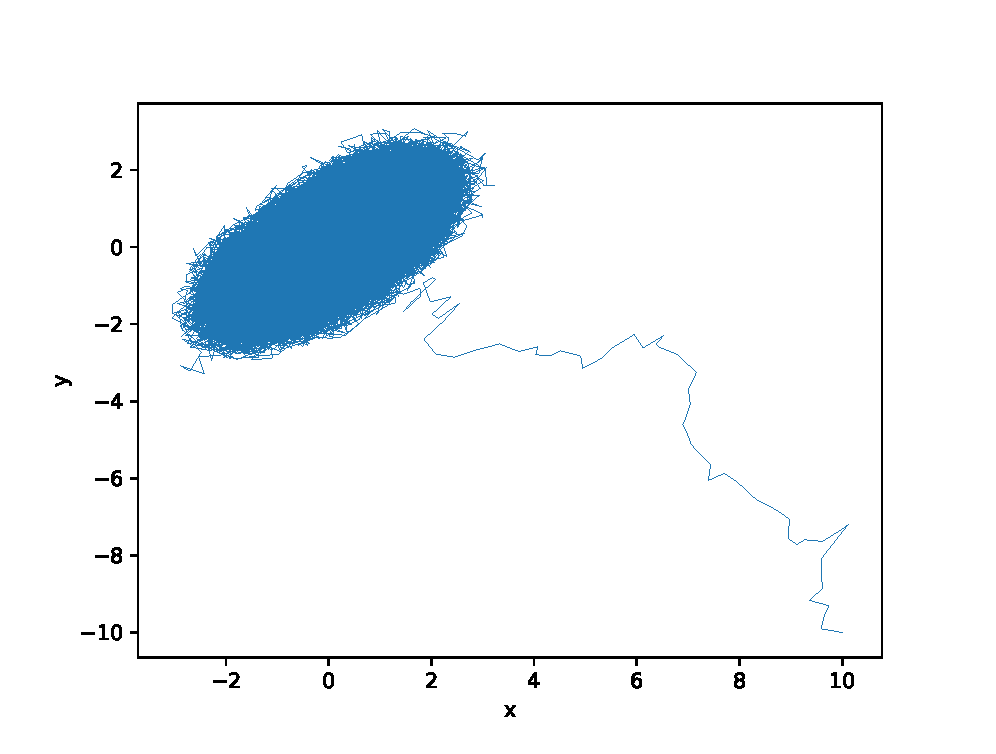
\includegraphics[width=0.5\textwidth]{0_2.eps}}
            \hfill
            \subfloat[抽样点分布图]{\includegraphics[width=0.5\textwidth]{0_2_1.eps}}
            \caption{$\beta=0.2$时Markov链点图($\Delta x = 1.0$)}
        \end{figure}
    \item $\beta=1.0$
        \begin{figure}[!h]
            \centering
            \subfloat[抽样点连线图]{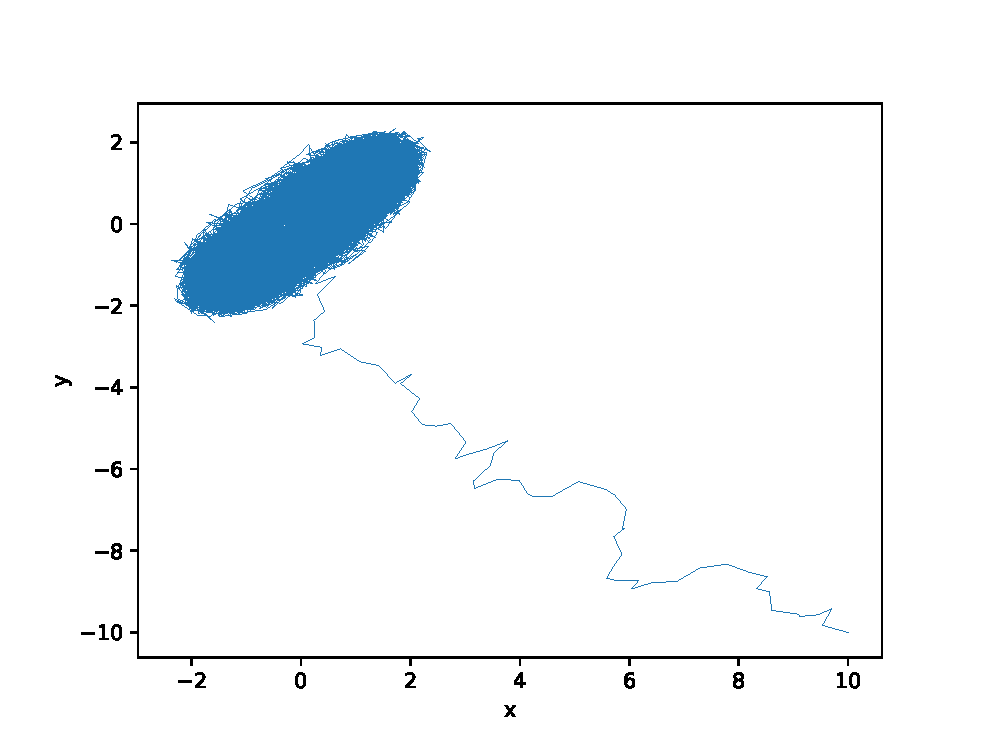
\includegraphics[width=0.5\textwidth]{1_0.eps}}
            \hfill
            \subfloat[抽样点分布图]{\includegraphics[width=0.5\textwidth]{1_0_1.eps}}
            \caption{$\beta=1.0$时Markov链点图($\Delta x = 1.0$)}
        \end{figure}
    \newpage
    \item $\beta=5.0$
        \begin{figure}[!h]
            \centering
            \subfloat[抽样点连线图]{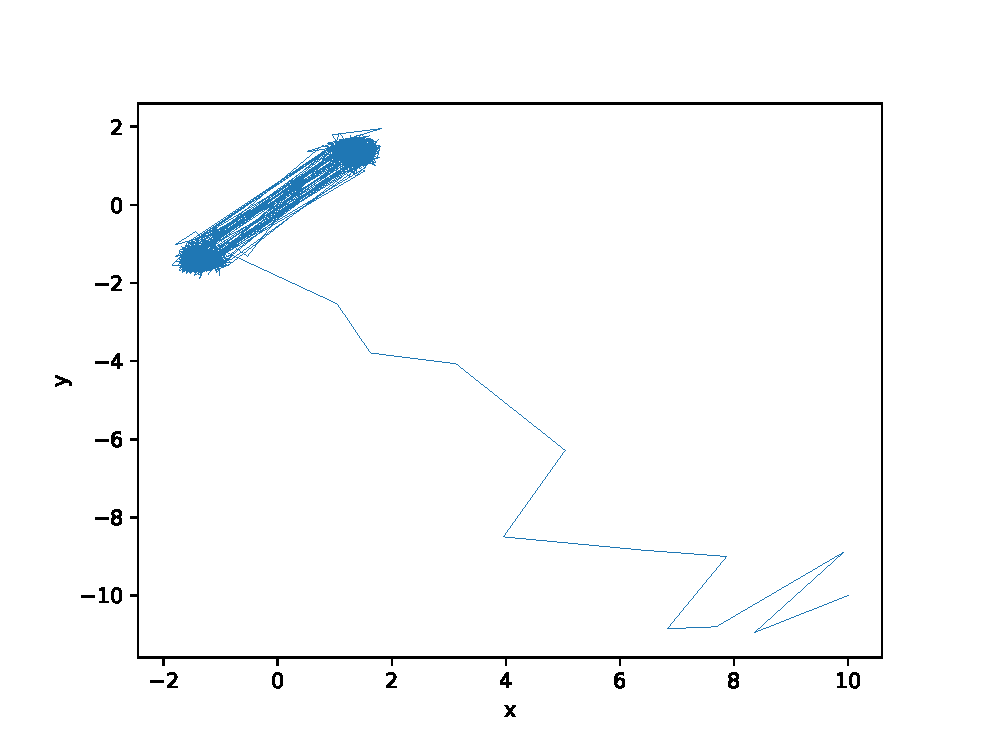
\includegraphics[width=0.5\textwidth]{5_0.eps}}
            \hfill
            \subfloat[抽样点分布图]{\includegraphics[width=0.5\textwidth]{5_0_1.eps}}
            \caption{$\beta=5.0$时Markov链点图($\Delta x = 5.0$)}
        \end{figure}

    所得积分值如下表:
\begin{table}[!h]
\centering
\caption{积分值计算结果}
\begin{tabular}{|l|l|l|l|}
\hline
$\beta$ & $\langle x^2\rangle$ & $\langle y^2\rangle$ & $\langle x^2+y^2\rangle$ \\ \hline
0.2     & 1.6242               & 1.5795               & 3.2038                   \\ \hline
1.0     & 1.7148               & 1.7283               & 3.4432                   \\ \hline
5.0     & 1.9650               & 1.9743               & 3.9394                   \\ \hline
\end{tabular}
\end{table}  
\end{itemize}
\section{结论}

本题我们进行了Metropolis方法的模拟(模拟退火法)并绘制了Markov链,对Markov链有了更深的理解.

\newpage
\section{源代码}
FORTRAN90源代码:
\begin{framed}
\begin{lstlisting}[language=Fortran]
MODULE Metropolis
IMPLICIT NONE
CONTAINS
    SUBROUTINE Sample(x0, y0, beta, num, step, filename)
        CHARACTER(LEN=*), INTENT(IN) :: filename
        REAL(KIND=8), INTENT(IN) :: beta, x0, y0, step
        REAL(KIND=8) :: rand(3 * num), xt(2), x(0:num, 2), d, seed
        INTEGER(KIND=4), INTENT(IN) :: num
        INTEGER(KIND=4) :: i
        x(0, 1) = x0
        x(0, 2) = y0 ! 初始化起步点
        CALL RANDOM_NUMBER(seed)
        ! 用FORTRAN自带的随机数生成器生成16807生成器的种子
        CALL Schrage(3 * num, int(2147483647 * seed), rand)
        DO i = 1, num
            xt(1) = x(i-1, 1) + step * (rand(i) - 0.5)
            xt(2) = x(i-1, 2) + step * (rand(2 * i) - 0.5) 
            ! xt储存建议的一步,是否接受取决于随机数的判断
            d = beta * (H(xt(1), xt(2)) - H(x(i-1, 1), x(i-1, 2))) ! 计算能量差d
            IF(d < 0) THEN
                x(i, :) = xt(:) ! 若能量减小则直接接收
            ELSE
                IF(rand(3 * i) < EXP(-d)) THEN
                    x(i, :) = xt(:) 
                    ! 若能量增加,使用rand(3*i)与Bolzmann因子EXP(-d)比较来进行判断
                ELSE
                    x(i, :) = x(i-1, :) 
                    ! 若前面两次判断都为假,则抽样失败,点与上一个点相同
                END IF
            END IF
        END DO
        OPEN (1, file=filename)
        WRITE (1, *) x
        CLOSE (1)
    END SUBROUTINE Sample
    
    SUBROUTINE Integrate(num, filename)
        CHARACTER(LEN=*) :: filename
        INTEGER(KIND=4) :: num
        INTEGER(KIND=4) :: i
        REAL(KIND=8), DIMENSION(0:num, 2) :: x
        REAL(KIND=8) :: i1, i2, i3
        OPEN (1, file=filename)
        READ (1, *) x
        CLOSE (1)
        i1 = 0
        i2 = 0
        i3 = 0
        DO i = 1, num
            i1 = real(i1 * (i-1)) / i + x(i, 1)**2 / i
            i2 = real(i2 * (i-1)) / i + x(i, 2)**2 / i
            i3 = real(i3 * (i-1)) / i + (x(i, 1)**2 + x(i, 2)**2) / i
            ! 按步更新平均值,可防止求和溢出
        END DO
        print *, 'i1 = ', i1
        print *, 'i2 = ', i2
        print *, 'i3 = ', i3
    END SUBROUTINE Integrate
    
    REAL(KIND=8) FUNCTION H(x, y)
        REAL(KIND=8), INTENT(IN) :: x, y
        H = -2 * (x**2 + y**2) + 0.5 * (x**4 + y**4) + 0.5 * (x - y)**4
    END FUNCTION H
END MODULE Metropolis   

SUBROUTINE Schrage(num, z0, rand)
    !Schrage随机数生成器子程序,将均匀随机数序列存放在数组rand中
    IMPLICIT NONE
    INTEGER(KIND=4) :: N = 1, num
    INTEGER :: m = 2147483647, a = 16807, q = 127773, r = 2836, In(num), z0
    REAL(KIND=8), INTENT(INOUT) :: rand(num)
    In(1) = z0 !将传入值z0作为种子
    rand(1) = REAL(In(1))/m
    DO N = 1, num - 1
        In(N + 1) = a * MOD(In(N), q) - r * INT(In(N) / q)
        IF (In(N + 1) < 0) THEN !若值小于零,按Schrage方法加m
            In(N + 1) = In(N + 1) + m
        END IF
        rand(N + 1) = REAL(In(N + 1))/m !得到第N+1个随机数
    END DO
END SUBROUTINE Schrage

PROGRAM MAIN
    USE Metropolis
    IMPLICIT NONE 
    CALL Sample(10.0_8, -10.0_8, 0.2_8, 100000, 1.0_8, '0_2.dat')
    print *, 'beta = 0.2:'
    CALL Integrate(100000, '0_2.dat')
    CALL Sample(10.0_8, -10.0_8, 1.0_8, 100000, 1.0_8, '1_0.dat')
    print *, 'beta = 1.0:'
    CALL Integrate(100000, '1_0.dat')
    CALL Sample(10.0_8, -10.0_8, 5.0_8, 100000, 5.0_8, '5_0.dat')
    print *, 'beta = 5.0:'
    CALL Integrate(100000, '5_0.dat')
END PROGRAM MAIN
\end{lstlisting}
\end{framed}

python绘图脚本代码:

\begin{framed}
\begin{lstlisting}[language=python]
import numpy as np
import matplotlib.pyplot as plt
import matplotlib as mpl
import math

plt.rcParams['savefig.dpi'] = 300
plt.rcParams['figure.dpi'] = 300

dat = np.loadtxt('0_2.dat')
x = dat[0:100000]
y = dat[100001:200001]
plt.xlabel('x')
plt.ylabel('y')
plt.plot(x, y, linewidth=0.1)
plt.savefig('0_2.eps')
plt.show()
plt.scatter(x, y, c=range(100000), cmap=mpl.cm.jet, s=0.1)
plt.colorbar(label="Counts", orientation='vertical')
plt.xlabel('x')
plt.ylabel('y')
plt.savefig('0_2_1.eps')
plt.show()

dat = np.loadtxt('1_0.dat')
x = dat[0:100000]
y = dat[100001:200001]
plt.xlabel('x')
plt.ylabel('y')
plt.plot(x, y, linewidth=0.1)
plt.savefig('1_0.eps')
plt.show()
plt.scatter(x, y, c=range(100000), cmap=mpl.cm.jet, s=0.1)
plt.colorbar(label="Counts", orientation='vertical')
plt.xlabel('x')
plt.ylabel('y')
plt.savefig('1_0_1.eps')
plt.show()

dat = np.loadtxt('5_0.dat')
x = dat[0:100000]
y = dat[100001:200001]
plt.xlabel('x')
plt.ylabel('y')
plt.plot(x, y, linewidth=0.1)
plt.savefig('5_0.eps')
plt.show()
plt.scatter(x, y, c=range(100000), cmap=mpl.cm.jet, s=0.1)
plt.colorbar(label="Counts", orientation='vertical')
plt.xlabel('x')
plt.ylabel('y')
plt.savefig('5_0_1.eps')
plt.show()
\end{lstlisting}
\end{framed}
\end{document}
